\begin{figure}
    \begin{subfigure}[b]{0.5\textwidth}
        \centering
        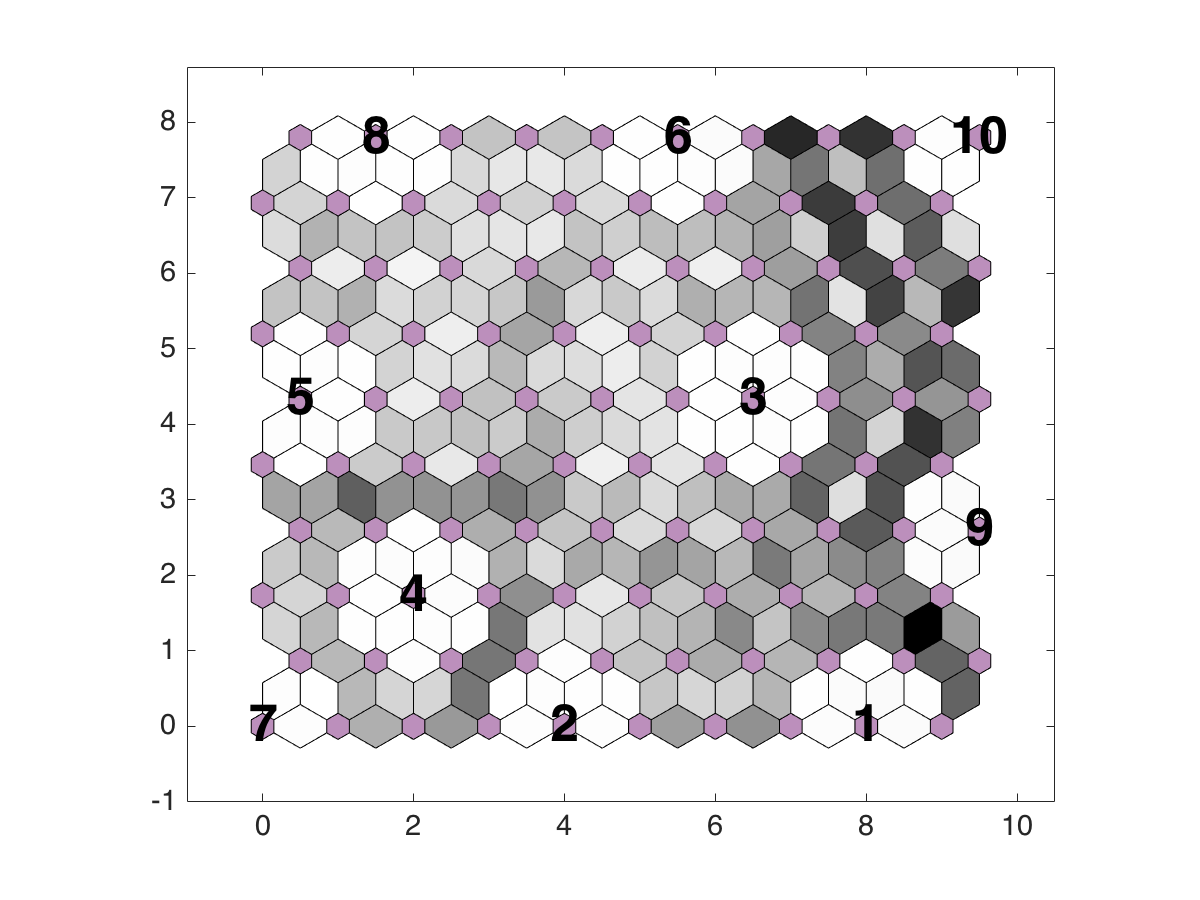
\includegraphics[width=\textwidth]{../../images0.01/M31/2D/diff_dimension/combine_2D_data_between_cols11and26.png}
    \caption{Without PAHs}
    \label{fig: wt_pahs}
    \end{subfigure}
    \hfill
    \begin{subfigure}[b]{0.5\textwidth}
        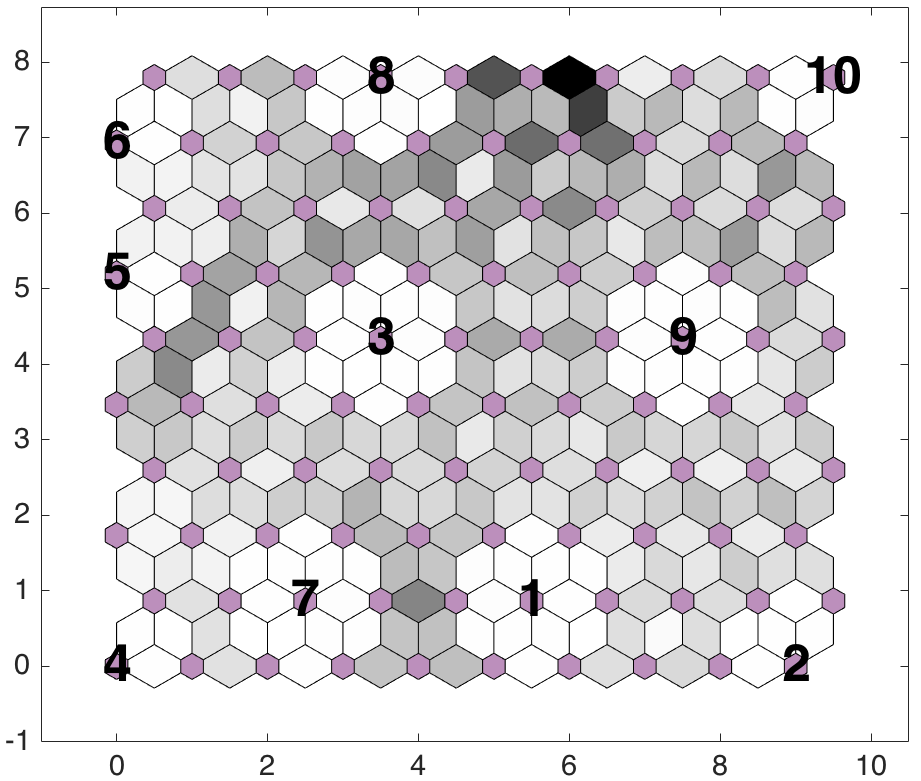
\includegraphics[width=\textwidth]{../../images0.01/M31/2D/diff_dimension/combine_2D_data_between_cols3and10.png}
    \caption{Only PAHs}
    \label{fig: only_pahs}
    \end{subfigure}
<<<<<<< HEAD
    \caption{Similar to Fig.~\ref{fig: all_derived_ones}, the self-organizing maps (top:) from data excluding PAHs; (bottom:) from PAH data only}
=======
    \caption{Similar to Fig.~\ref{fig: all_derived_ones}, here we show the result of up: SOM from data excluding PAHs; down: SOM from PAHs data.}
>>>>>>> sharelatex-2016-07-26-1530
    \label{fig: PAHS_or_not_PAHs}
\end{figure}
